\section{Empirical evaluation}
\label{sec:evaluation}

In the previous section, we showed that Spectral Experts provides a consistent
estimator.  %that converges a $\frac{1}{\sqrt n}$
In this section, we explore the empirical properties of our algorithm on simulated data.
Our main finding is that Spectral Experts alone attains higher parameter error than EM,
but this is not the complete story.
If we initialize EM with the estimates returned by Spectral Experts,
then we end up with much better estimates than EM from a random initialization.
%In this section, we will support these theoretical results with
%experiments on simulated data.
%We will see that in the finite sample
%regime, even when Spectral Experts does not converge to the optimal
%answer, it provides robust initialization for local methods like EM.

\subsection{Experimental setup}

\paragraph{Algorithms}

We experimented with three algorithms.
The first algorithm (Spectral) is simply the Spectral Experts.
We set the regularization strengths $\lambda_n^{(2)} = \frac{1}{10^{5} \sqrt{n}}$
and $\lambda_n^{(3)} = \frac{1}{10^{3} \sqrt{n}}$;
the algorithm was not very sensitive to these choices.
We solved the low-rank regression to estimate $M_2$ and
$M_3$ using an off-the-shelf convex optimizer, CVX~\cite{cvx}.
%ainterior point method an interior proximal subgradient descent
%algorithm.%\cite{candes11phaselift,tomioka2010estimation}. (Note sure about this citation and not required?)
%The algorithm was initialized with the regularized least squares
%solution and was run for 500 iterations or until convergence up to
%a tolerance of $10^{-3}$.
%Both regularization parameters, $\lambda_n^{(2)}$ and, $\lambda_n^{(3)}$ were annealed as $\frac{1}{n}$. 
The second algorithm (EM) is EM where the $\beta$'s are initialized from a standard normal
and $\pi$ was set to the uniform distribution plus some small perturbations.
We ran EM for 1000 iterations.
In the final algorithm (Spectral+EM),
we initialized EM with the output of Spectral Experts.

\paragraph{Data}

We generated synthetic data as follows:
First, we generated a vector $t$ sampled uniformly over the $b$-dimensional
unit hypercube $[-1,1]^b$.
Then, to get the actual covariates $x$, we applied a non-linear function of $t$
that conformed to the identifiability criteria discussed in
\sectionref{sec:algo}.
The true regression coefficients $\{\beta_h\}$ were drawn from a standard normal
and $\pi$ is set to the uniform distribution.
The observation noise $\epsilon$ is drawn from a normal with variance $\sigma^2$.
Results are presented below for $\sigma^2 = 0.1$, but we did not observe any
qualitatively different behaviour for choices of $\sigma^2$ in the range
$[0.01, 0.4]$.  

As an example, one feature map we considered in the one-dimensional
setting $(b=1)$ was $x = (1, t, t^4, t^7)$. The data and the curves fit using
Spectral Experts, EM with random initialization and EM initialized with
the parameters recovered using Spectral Experts are shown in
\figureref{fig:curves}. We note that even on well-separated data such as
this, EM converged to the correct basin of attraction only 13\% of the time.

\begin{figure}[t]
  \centering
  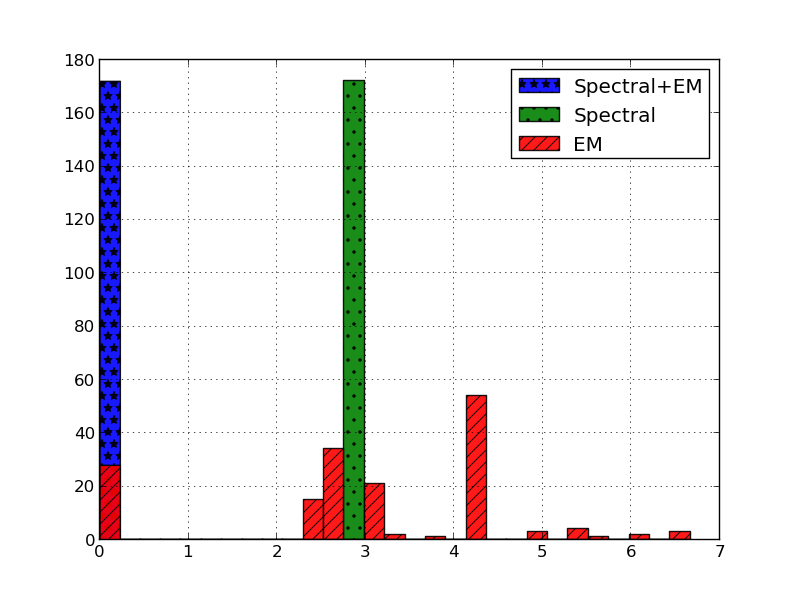
\includegraphics[width=0.50\textwidth]{figures/hist.png}
  \caption{Histogram over recovery errors between the three algorithms when $b = 1, d = 4, k = 3, n = 500,000$.}
  \label{fig:hist}
\end{figure}


\begin{figure*}[p]
  \centering
  \subfigure[Spectral, Spectral+EM]{
    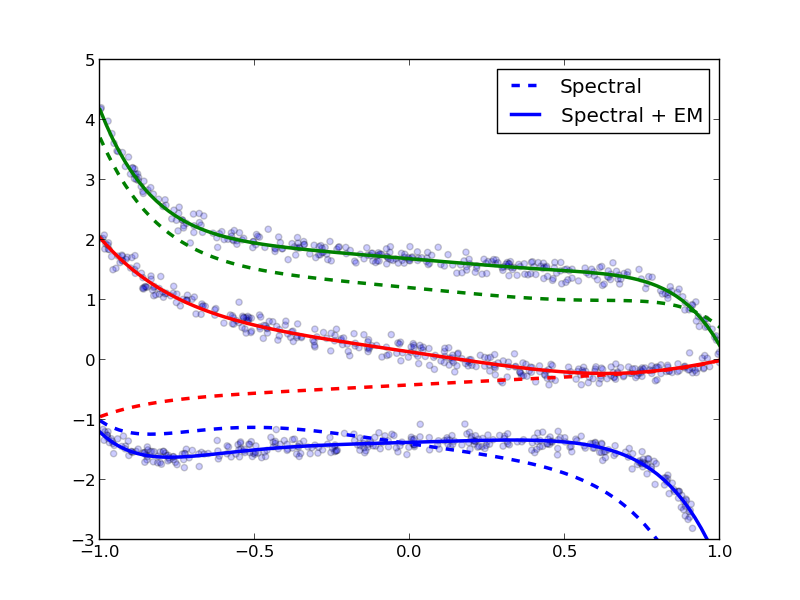
\includegraphics[width=0.50\textwidth]{figures/curves-vis/1-8-3-specm.png}}
    \hspace{-2em}
  \subfigure[EM]{
    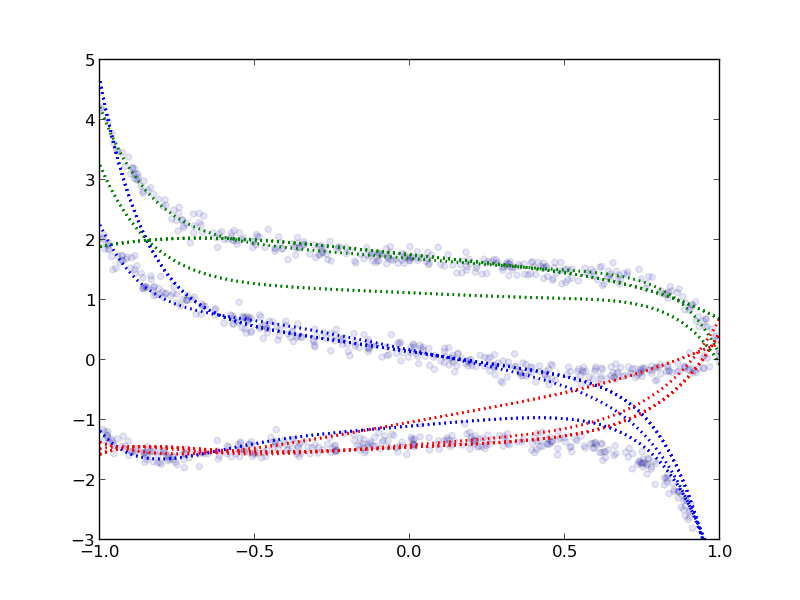
\includegraphics[width=0.50\textwidth]{figures/curves-vis/1-8-3-em.png}}
%  \subfigure[Spectral + EM]{
%    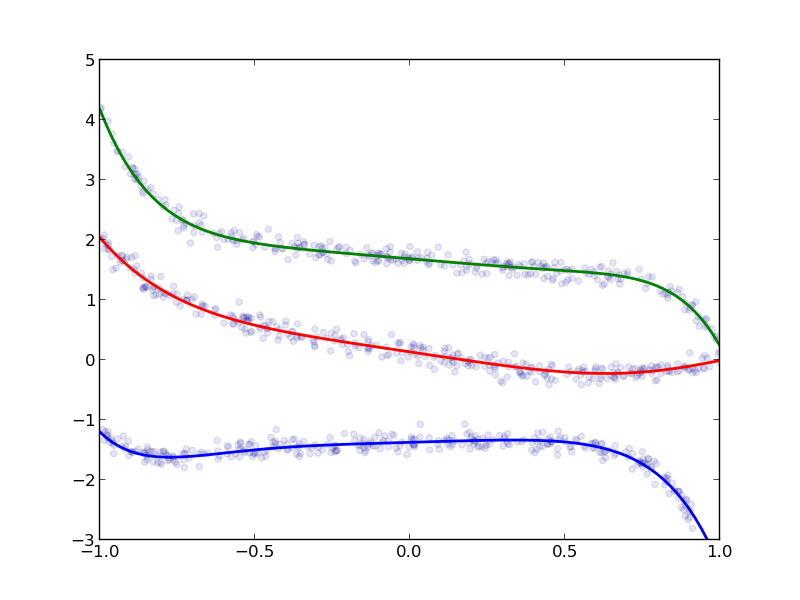
\includegraphics[width=0.34\textwidth]{figures/curves-vis/1-8-3-spem.png}}
  \caption{Visualization of the parameters estimated by Spectral Experts versus EM.
  (a) The dashed lines denote the solution recovered by Spectral Experts. While
  not a perfect fit, it provides an good initialization for EM to further improve the solution (solid lines).
  (b) The dotted lines show different local optima found by EM.}
  \label{fig:curves}
\end{figure*}

%Default values:
%$n = 10^6$
%$k = 5$

\begin{table*}[tbhp]
\caption{Parameter error $\|\theta^* - \hat \theta\|_F$ ($n = 500,000$)
as the number of base variables $b$, number of features $d$ and the number of components $k$ increases.
While Spectral by itself does not produce good parameter estimates, Spectral+EM improves
over EM significantly.
}
\label{tbl:parameter-recovery}
\vskip 0.15in
\begin{center}
\begin{small}
\begin{sc}

  \begin{tabular}{ r r r c c c }
\hline
\abovespace\belowspace
Variables ($b$) & Features ($d$) & Components ($k$) & Spectral & EM & Spectral + EM \\
\hline
\abovespace
%$\{1$, $ x_1$, $ x_1^4\}$ 
  1 & 4 & 2 & 2.45 $\pm$ 3.68 & 0.28 $\pm$ 0.82 & {\bf 0.17 $\pm$ 0.57} \\
% 1-5-2 2.451423 (+/- 3.686348) 0.176685 (+/- 0.579108) 0.007634 (+/- 0.001706) 0.341620 (+/- 0.584178) 0.010296 (+/- 0.007839)
%$\{1$, $ x_1$, $ x_2$, $ x_1^2 x_2^2\}$ 
2 & 5 & 2 & 1.38 $\pm$ 0.84 & {\bf 0.00 $\pm$ 0.00} & {\bf 0.00 $\pm$ 0.00} \\
% 2-3-2 1.383626 (+/- 0.840325) 0.001416 (+/- 0.000083) 0.003312 (+/- 0.000399) 0.454076 (+/- 0.758689) 0.003340 (+/- 0.000397)
  2 & 5 & 3 & 2.92 $\pm$ 1.71 & 0.43 $\pm$ 1.07 & {\bf 0.31 $\pm$ 1.02} \\
% 2-3-3 2.917581 (+/- 1.714054) 0.308649 (+/- 1.024135) 0.003885 (+/- 0.000442) 0.661009 (+/- 0.543162) 0.012455 (+/- 0.033185)
%$\{1$, $ x_1$, $ x_2$, $ x_1 x_2^3$, $ x_1^2 x_2^2$, $ x_1^3 x_2 \}$ 
  2 & 6 & 2 & 2.33 $\pm$ 0.67 & 0.63 $\pm$ 1.29 & {\bf 0.01 $\pm$ 0.01} \\
% 2-4-2 2.333000 (+/- 0.674578) 0.004067 (+/- 0.001391) 0.001167 (+/- 0.001096) 0.592667 (+/- 0.478518) 0.001200 (+/- 0.001143)
%\belowspace
%  2 & 6 & 5 & 6.78 $\pm$ 2.18 & 2.29 $\pm$ 1.79 & {\bf 1.77 $\pm$ 1.89} \\

%  2 & 5 & 3 & 1.87 $\pm$ 1.20 & {\bf 0.33 $\pm$ 0.96} & 0.35 $\pm$ 1.23 \\
% 2 & 6 & 5 & 5.27 $\pm$ 2.32 & 1.80 $\pm$ 1.80 & {\bf 1.51 $\pm$ 1.77} \\
%$\{1$, $ x_1$, $ x_2$, $ x_1 x_2^3$, $ x_1^2 x_2^2$, $ x_1^3 x_2$, $ x_1^3 x_2^4$, $ x_1^4 x_2^3 \}$ 
% 2 & 8 & 7 & 8.42 $\pm$ 1.66 & 7.41 $\pm$ 2.99 & {\bf 7.31 $\pm$ 2.47} \\
%$\{1$, $ x_1$, $ x_2$, $ x_3$, $ x_1 x_2 x_3^2$, $ x_1 x_2^2 x_3$, $ x_1^2 x_2 x_3$, $ x_1^2 x_2^2$, $ x_1^2 x_3^2$, $ x_2^2 x_3^2$, $ x_3^2\}$
% 3 & 10 & 3 & 3.78 $\pm$ 0.90 & 0.67 $\pm$ 1.49 & {\bf 0.51 $\pm$ 1.12} \\
%$\{1$, $ x_1$, $ x_2$, $ x_3$, $ x_1 x_2 x_3^2$, $ x_1 x_2^2 x_3$, $ x_1^2 x_2 x_3$, $ x_1^2 x_2^2$, $ x_1^2 x_3^2$, $ x_2^2 x_3^2$, $ x_3^2\}$
% 3 & 10  & 7 & 9.97 $\pm$ 3.22 & 1.43 $\pm$ 1.97 & {\bf 1.42 $\pm$ 2.17} \\

\hline

\end{tabular}
\end{sc}
\end{small}
\end{center}
\vskip -0.1in
\end{table*}

% \todo{Dataset 2: $b = 30$, $p = 1$. I'm unclear as to what we can show
% on this sort of data set. EM works extremely well, and the spectral
% methods do not converge easily.}

\begin{figure*}[tbhp]
  \centering
  \subfigure[Well-specified data]{
    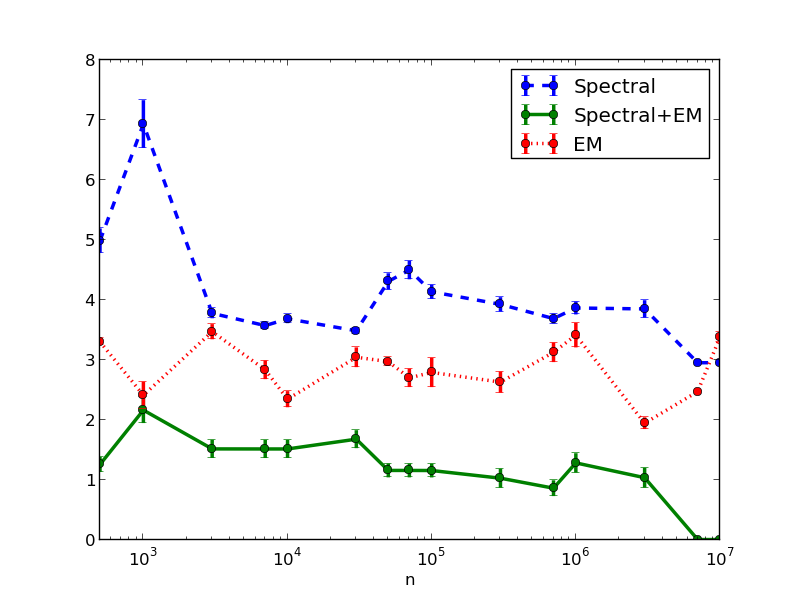
\includegraphics[width=0.50\textwidth]{figures/vs-n/1833-decay.png}
  }
    \hspace{-2em}
  \subfigure[Misspecified data]{
    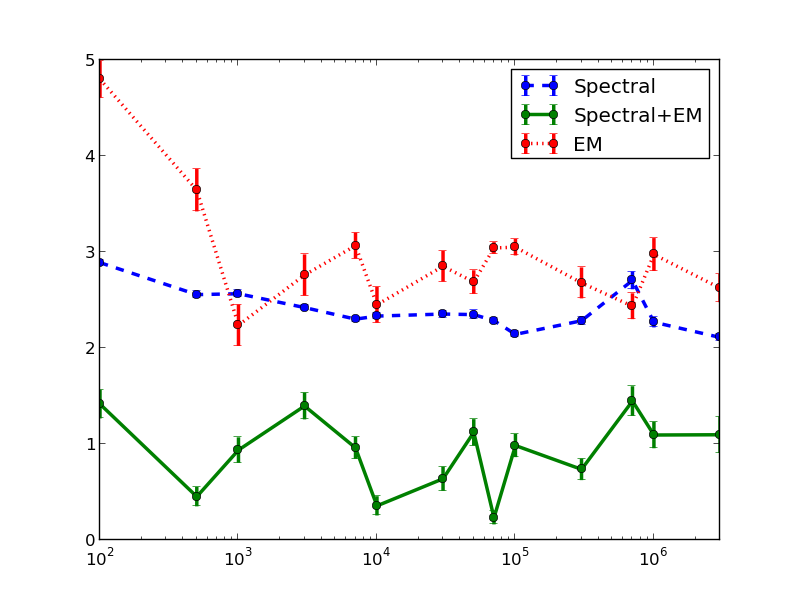
\includegraphics[width=0.50\textwidth]{figures/vs-n/1-8-3-3-rm.png}
  }
  \caption{Learning curves: parameter error as a function of the number of samples $n$ ($b = 1, d = 5, k = 3$).}
  \label{fig:vs-n}
\end{figure*}


\subsection{Results}

\begin{table*}[tbhp]
\caption{Parameter error $\|\theta^* - \hat \theta\|_F$ when the data is misspecified ($n = 500,000$).
Spectral+EM degrades slightly, but still outperforms EM overall.
}
\label{tbl:parameter-recovery-mis}
\vskip 0.15in
\begin{center}
\begin{small}
\begin{sc}

  \begin{tabular}{ r r r c c c }
\hline
\abovespace\belowspace
Variables ($b$) & Features ($d$) & Components ($k$) & Spectral & EM & Spectral + EM \\
\hline
\abovespace
 1 & 4 & 2 &  1.55 $\pm$ 0.84 & 0.29 $\pm$ 0.85 &  {\bf 0.01 $\pm$ 0.07} \\
 % 1-5-2 1.553269 (+/- 0.841002) 0.008463 (+/- 0.067282) 0.006283 (+/- 0.007291) 0.700833 (+/- 1.650770) 0.006344 (+/- 0.007351) 0.124876 (+/- 0.145539) 2.304894 (+/- 2.457321)
%\belowspace
 2 & 5 & 3 &  1.37 $\pm$ 0.85 & 0.44 $\pm$ 1.12 &  {\bf 0.00 $\pm$ 0.00} \\
% 2-3-2 1.373689 (+/- 0.849721) 0.002074 (+/- 0.000116) 0.004720 (+/- 0.000000) 0.501348 (+/- 0.656840) 0.004702 (+/- 0.000009)
 2 & 6 & 5 &  9.89 $\pm$ 4.46 & {\bf 2.53 $\pm$ 1.77} &  2.69 $\pm$ 1.83 \\
 2 & 8 & 7 & 23.07 $\pm$ 7.10 & 9.62 $\pm$ 1.03 &  {\bf 8.16 $\pm$ 2.31}  \\
\hline

\end{tabular}
\end{sc}
\end{small}
\end{center}
\vskip -0.1in
\end{table*}


\tableref{tbl:parameter-recovery} presents the Frobenius norm of the
difference between true and estimated parameters for the model, averaged
over 20 different random instances for each feature set and 10 attempts
for each instance. The experiments were run using $n = 500,000$ samples.

One of the main reasons for the high variance is the variation across
random instances; some are easy for EM to find the global minima and
others more difficult. In general, while Spectral Experts did not
recover parameters by itself extremely well, it provided a good initialization for
EM.

To study the stability of the solutions returned by Spectral Experts,
consider the histogram in \figureref{fig:hist}, which shows the recovery
errors of the algorithms over 170 attempts on a dataset with $b = 1, d = 4,
k = 3$. Typically, Spectral Experts returned a stable solution.
When these parameters were close enough to the true parameters, we found
that EM almost always converged to the global optima. Randomly
initialized EM only finds the true parameters a little over 10\% of the
time and shows considerably higher variance. 

\paragraph{Effect of number of data points}

In \figureref{fig:vs-n}, we show how the recovery error varies as we get
more data. Each data point shows the mean error over 10 attempts, with
error bars. We note that the recovery performance of EM does not
particularly improve; this suggests that EM continues to get stuck in
a local optima. The spectral algorithm's error decays slowly, and as it
gets closer to zero, EM initialized at the spectral parameters finds the
true parameters more often as well. This behavior highlights the
trade-off between statistical and computational error. 

\paragraph{Misspecified data}

To evaluate how robust the algorithm was to model mis-specification, we
removed large contiguous sections from $x \in [-0.5,-0.25] \cup
[0.25,0.5]$ and ran the algorithms again.
\tableref{tbl:parameter-recovery-mis} reports recovery errors in this
scenario. The error in the estimates grows larger for higher $d$.

